\documentclass[tikz,border=2mm]{standalone}

\begin{document}

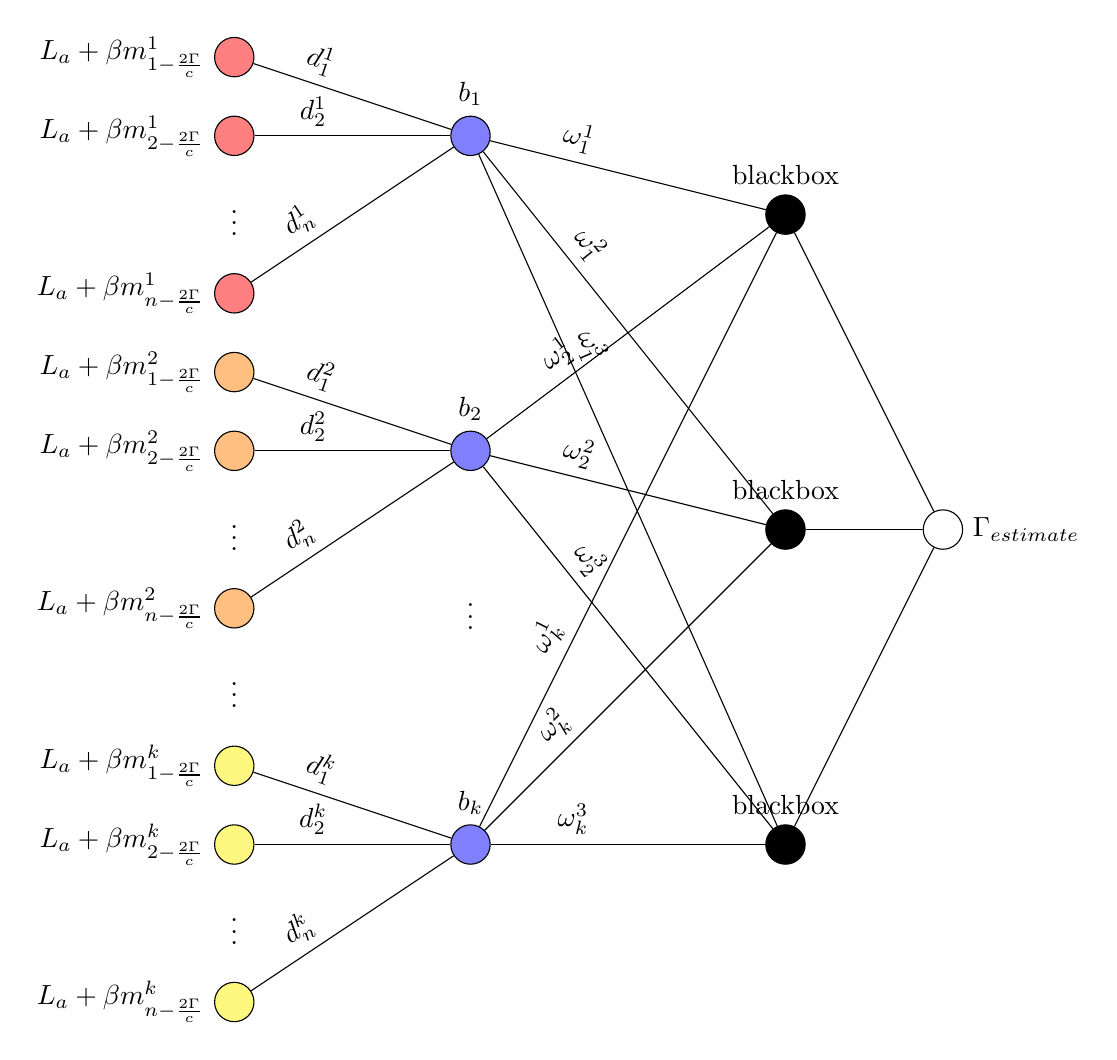
\begin{tikzpicture}
[   cnode/.style={draw=black,fill=#1,minimum width=5mm,circle},
]
    %
    \node[cnode=white,label=0:$\Gamma_{estimate}$] (output) at (9,-7) {};
    \node[cnode=black,label=90:blackbox] (s1) at (7,-3) {};
    \draw (s1) -- node[above,sloped,pos=0.3] {} (output);
    \node[cnode=black,label=90:blackbox] (s2) at (7,-7) {};
    \draw (s2) -- node[above,sloped,pos=0.3] {} (output);
    \node[cnode=black,label=90:blackbox] (s3) at (7,-11) {};
    \draw (s3) -- node[above,sloped,pos=0.3] {} (output);
    \node at (0,-3) {$\vdots$};
    \node at (0,-7) {$\vdots$};
    \node at (0,-9) {$\vdots$};
    \node at (0,-12) {$\vdots$};
    
    \node at (3,-8) {$\vdots$};

    \foreach \k in {1,...,3}
    {   
        \pgfmathparse{\k<3 ? \k : "k"} % If x < 4 then give it its value, else give it the value N
        \node[cnode=blue!50,label=90:$b_{\pgfmathresult}$] (b-\k) at (3,{-\k-div(\k,3) - 3*\k + 2}) {};
        \draw (b-\k) -- node[above,sloped,pos=0.3] {$\omega^{1}_{\pgfmathresult}$} (s1);
        \draw (b-\k) -- node[above,sloped,pos=0.3] {$\omega^{2}_{\pgfmathresult}$} (s2);
        \draw (b-\k) -- node[above,sloped,pos=0.3] {$\omega^{3}_{\pgfmathresult}$} (s3);
    }
  
    \foreach \x in {1,...,3}
    {   
        \pgfmathparse{\x<3 ? \x : "n"} % If x < 4 then give it its value, else give it the value N
        \node[cnode=red!50,label=180:$L_a + \beta m^{1}_{\pgfmathresult - \frac{2\Gamma}{c}}$] (m1-\x) at (0,{-\x-div(\x,3)}) {};
        \draw (m1-\x) -- node[above,sloped,pos=0.3] {$d^{1}_{\pgfmathresult}$} (b-1);
    }
    \foreach \x in {1,...,3}
    {   
        \pgfmathparse{\x<3 ? \x : "n"} % If x < 4 then give it its value, else give it the value N
        \node[cnode=orange!50,label=180:$L_a + \beta m^{2}_{\pgfmathresult - \frac{2\Gamma}{c}}$] (m2-\x)  at (0,{-\x-div(\x,3) - 4}) {};
        \draw (m2-\x) -- node[above,sloped,pos=0.3] {$d^{2}_{\pgfmathresult}$} (b-2);
    }
    \foreach \x in {1,...,3}
    {   
        \pgfmathparse{\x<3 ? \x : "n"} % If x < 4 then give it its value, else give it the value N
        \node[cnode=yellow!50,label=180:$L_a + \beta m^{k}_{\pgfmathresult - \frac{2\Gamma}{c}}$] (mk-\x) at (0,{-\x-div(\x,3) - 9}) {};
        \draw (mk-\x) -- node[above,sloped,pos=0.3] {$d^{k}_{\pgfmathresult}$} (b-3);
    }



    % \foreach \x in {1,...,4}
    % {   \foreach \y in {1,...,4}
    %     {   
    %         \draw (x-\x) -- (p-\y);
    %     }
    % }
\end{tikzpicture}

\end{document}